% 第 7 周交付物:扩展敏感性分析报告(中文版) —— 编译方式:XeLaTeX
\documentclass[11pt]{ctexart}
\usepackage[a4paper, margin=2.4cm]{geometry}
\usepackage{amsmath}
\usepackage{booktabs}
\usepackage{graphicx}
\usepackage[hidelinks]{hyperref}
\usepackage{enumitem}
\setlist{nosep}

\title{\textbf{扩展敏感性分析报告}\\
\large Advanced Chooser Option Pricing Model --- 第 7 周交付物}
\author{佟铸城 (Zhucheng Tong)}
\date{2026 年 8 月(市场快照:2026-08-20)}

\begin{document}
\maketitle

\section{分析基准}
以最新交易日(2026-08-20,自动化管道数据)为市场快照:$S=\$351.55$、$\sigma_{EWMA}=19.1\%$、$r_{1y}=3.99\%$、$q=1.71\%$,市场状态判定为\textbf{平静}(VIX 分位 $<0.75$)。基准合约为 ATM 1 年期 chooser($t_1=0.5$),主定价 \$44.82,误差区间 $\pm$\$9.01(第 4 周平静状态基准 MAE)。

\section{极端情景测试(含任务书规格:波动率 $+50\%$、加息 200bp)}
\begin{center}
\small
\begin{tabular}{lrrr}
\toprule
\textbf{情景} & \textbf{价格(\$)} & \textbf{变化(\$)} & \textbf{变化(\%)} \\
\midrule
基准(当前市场) & 44.82 & --- & --- \\
波动率 $+50\%$ & 66.76 & $+21.94$ & $+48.9$ \\
波动率 $-30\%$ & 31.72 & $-13.10$ & $-29.2$ \\
利率 $+200$bp & 45.49 & $+0.67$ & $+1.5$ \\
利率 $-100$bp & 44.74 & $-0.08$ & $-0.2$ \\
股价 $-15\%$($K$ 不变) & 55.47 & $+10.65$ & $+23.8$ \\
股价 $+15\%$($K$ 不变) & 70.04 & $+25.22$ & $+56.3$ \\
组合压力(波动率$+50\%$ 且 利率$+200$bp) & 66.84 & $+22.02$ & $+49.1$ \\
\bottomrule
\end{tabular}
\end{center}

三个解读:(1) \textbf{波动率是绝对主导因子}:$+50\%$ 波动率抬价近半,而 200bp 加息只抬价 1.5\%——chooser 双腿的 vega 同向叠加、rho 反向抵消(call 腿 $+$、put 腿 $-$),这是它区别于单腿期权的结构特征;(2) \textbf{对股价双向凸性}:现价上下 15\% 都使价格上升(向上 call 腿获益更大,不对称源于对数正态漂移),印证第 3 周"chooser 对 $K$ 呈 U 形"的敏感性结论;(3) \textbf{组合压力 $\approx$ 单因子波动率压力}:利率冲击在 chooser 上近乎中性,压力测试的关注点应集中于波动率维度。

\begin{figure}[h!]
\centering
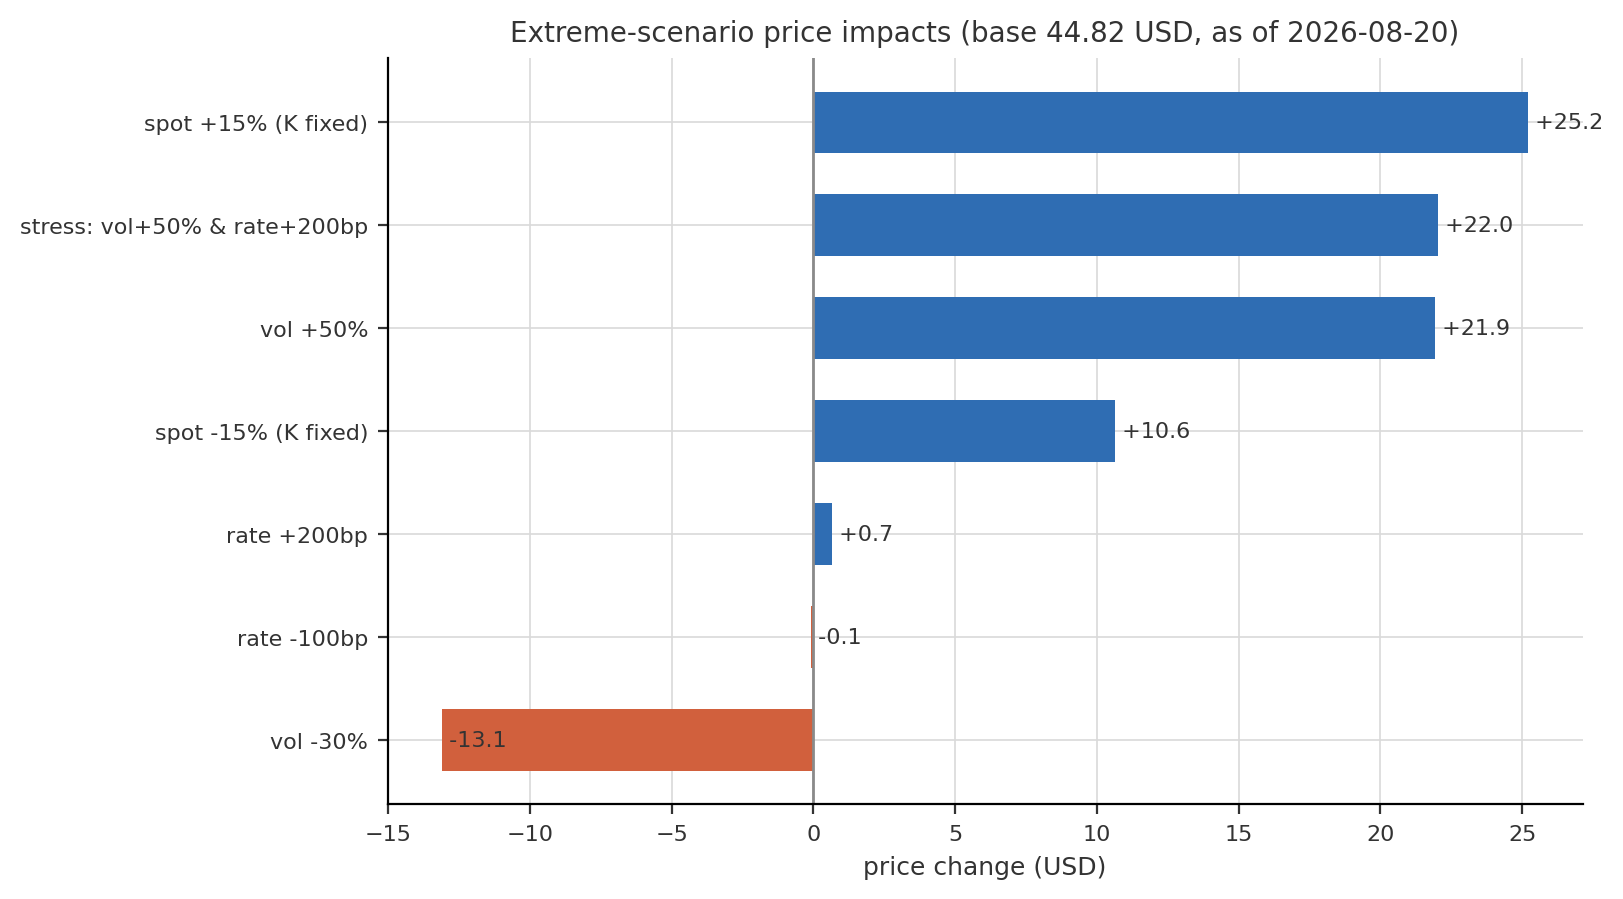
\includegraphics[width=0.8\textwidth]{figures/scenario_tornado.png}
\caption{极端情景的价格冲击(美元)}
\end{figure}

\begin{figure}[h!]
\centering
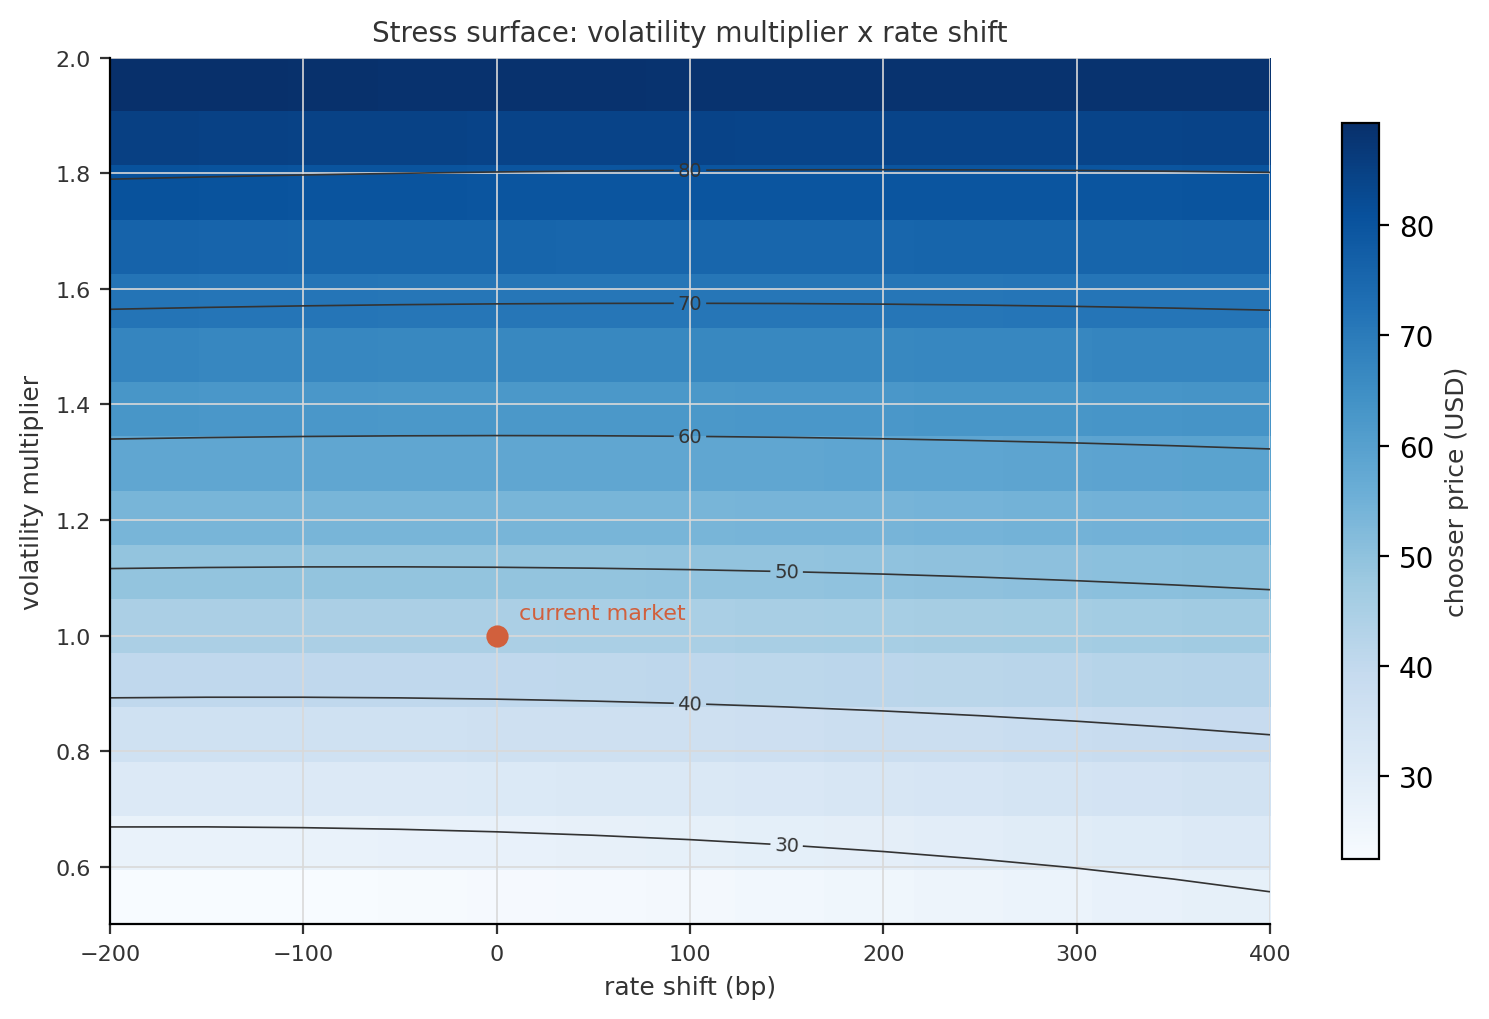
\includegraphics[width=0.74\textwidth]{figures/stress_heatmap.png}
\caption{压力曲面:波动率乘数 $\times$ 利率平移(等高线为价格)}
\end{figure}

\section{SHAP 特征影响的美元化(任务书:量化新特征的影响)}
把第 6 周 SHAP 对 $\ln\sigma$ 的平均绝对贡献,经定价函数映射为当前市场下的\textbf{美元价格影响}:一次典型幅度的特征贡献,对应的价格变化为——\texttt{realized\_vol\_252d} $+\$16.94$、\texttt{realized\_vol\_63d} $+\$7.72$、\texttt{beta\_63d} $+\$5.59$、\texttt{realized\_vol\_21d} $+\$3.71$、\texttt{div\_growth\_yoy} $+\$3.48$;VIX 系特征(水平/分位/动量)单次贡献均 $<\$2$。解读:在锚定(相对 EWMA)口径下,\textbf{长记忆波动率信息主导修正方向}——VIX 的水平信息已被锚吸收,其增量贡献自然变小,这与第 2 周(预测波动率水平时 VIX 主导)并不矛盾,恰好说明锚定设计成功剥离了已知结构。

\begin{figure}[h!]
\centering
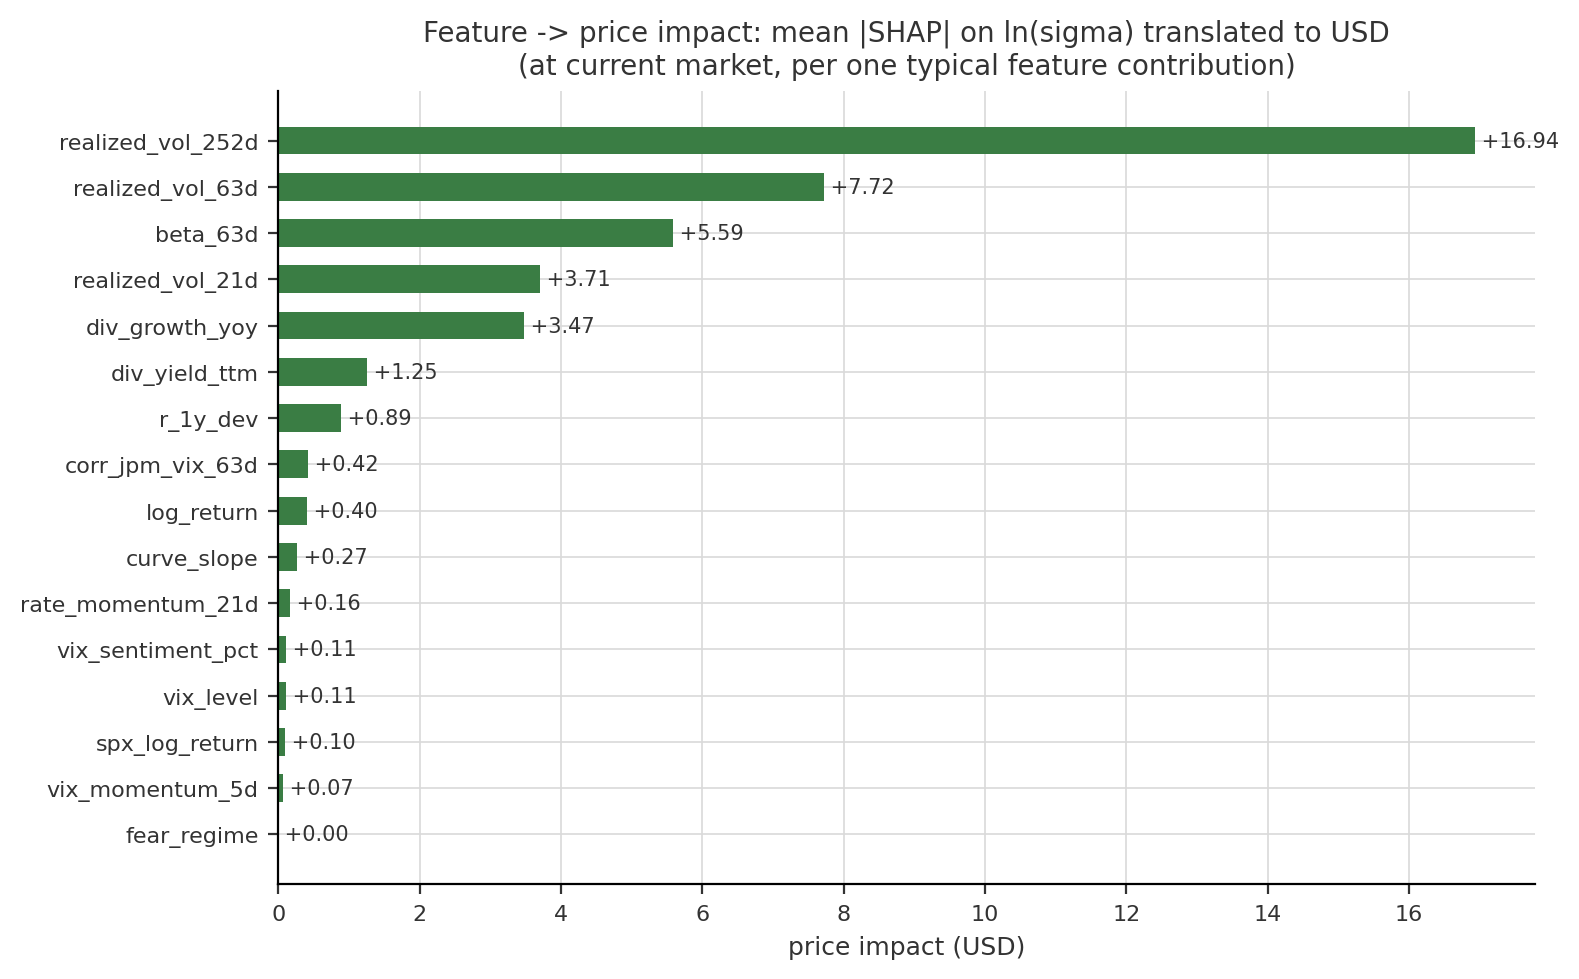
\includegraphics[width=0.72\textwidth]{figures/shap_price_impact.png}
\caption{特征 $\to$ 价格影响(美元,当前市场快照)}
\end{figure}

\section{定价工具原型与实时数据集成(本周另两项交付)}
Streamlit 工具(\texttt{streamlit run app/streamlit\_app.py})已实现:双定价(EWMA 锚定 BSM 主价 + ML 参考价带样本外警示)、分状态误差区间、价格趋势、情景与波动率敏感性、第 4/6 周性能指标存档;\textbf{实时数据}:侧栏一键拉取(复用采集管道,\texttt{END\_DATE=当日}),另有 GitHub Actions 每周五自动更新。全部定价逻辑位于独立的 \texttt{src/tool/pricing\_service.py},六项审计(闭式解一致、无套利排序、情景重算、压力面单调、确定性、UI 零公式)全部通过。

\end{document}
